\section{Comparison against SQLite}

\subsection{Test methodology}

To compare the LSM solution with SQLite, a simple storage system was developed. It has a database that consists of two tables. The first table is called Measurement and it is used to store the measurements. Each measurement is represented by its key, timestamp and value, while the key is the primary ID of MeasurementMeta entity, that is stored in the second table. This entity stores the tag name of the measurement; therefore it is possible to perform search operations filtering by numeric column instead of a text column. The Measurement table has indexes on both the key and the timestamp columns.

For the following benchmarks, a sample synthetic setup was used. This setup has 10 sensors that emit data at a sampling frequency of 1Hz. For the reading benchmarks, the data for those 10 tags were generated for the time range of three hours. Therefore, the SQLite database had 108000 entries, or points, in total, which means 10800 points per each tag. The LSM library has 108000 entries as well, splitted across 10 files per each tag, having 10800 points in each one. For the writing benchmarks, the data for those 10 tags is generated for various time ranges and then stored in both storage engines.

In order to benchmark both storage engines, a standard Go benchmarking mechanism was used. It runs the target code multiple times until the benchmark function lasts long enough to be measured reliably~\cite{go_benchmark}. It produces the result that is measured in ns/op, nanoseconds per iteration; for the following benchmarks, iteration is a single storage read or storage write call.

All benchmarks were running on a PC with Intel Core i5-8400 running Ubuntu 18.04, the data files for both storages were stored on an NVMe SSD.

\subsection{Reading from full range of data}

This benchmark measures the read time for various time ranges, while the operation is performed across full three hours of measurements. The results of this benchmark are available in Figure~\ref{fig3}. As seen, the GoLSM is about twice as fast as SQLite engine on read requests. It is worth mentioning that the $C_0$ level of LSM tree is not playing a significant role in speeding up the data retrieval, since the time range is picked randomly from across all three hours of measurements while the $C_0$ level only contains the last two minutes of measurements.

\begin{figure}[h!]
	\centering
	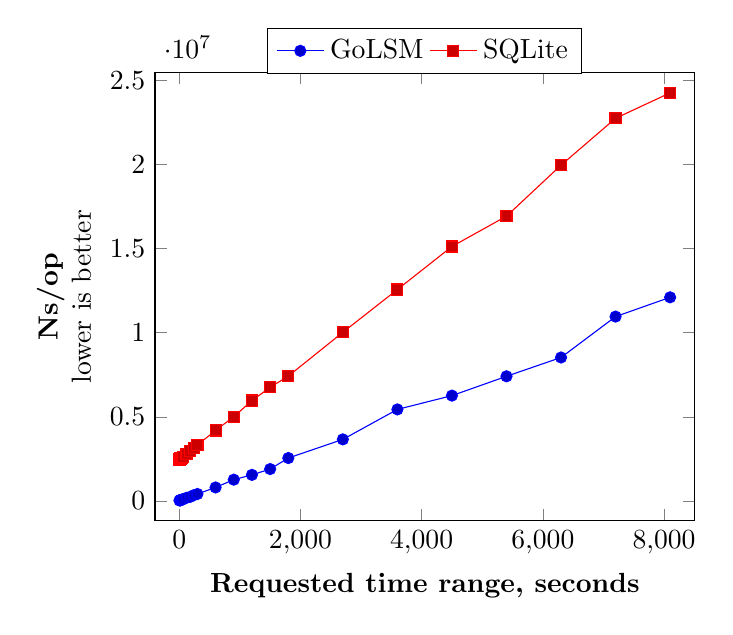
\begin{tikzpicture}
        % first provide your data as table, so later the data can
        % easily be accessed for various stuff
        \pgfplotstableread{
            x    y  z
5 29245				    2468624
10 34331			    2488443
15 41885			    2487442
20 47359			    2533488
25 51261			    2517353
30 62037			    2529031
45 76538			    2571565
60 101490			    2611909
120 185574			    2787438
180 241142			    2986666
240 341329			    3155070
300 412849			    3327132
600 801901			    4190652
900 1264738			    5008636
1200 1549898			    5966411
1500 1895210			    6753930
1800 2550300			    7420697
2700 3659991			    10027510
3600 5442224			    12570023
4500 6261830			    15128483
5400 7410561			    16932040
6300 8529041			    19965360
7200 10960360			    22752193
8100 12106688			    24262132
        }{\data}
    \begin{axis}[
        x tick style={/pgf/number format/1000 sep=},
	    ylabel style={align=center},	
	    ylabel = \textbf{Ns/op}\\lower is better,
	    xlabel style={align=center},	
	    xlabel = \textbf{Requested time range, seconds},
	    enlargelimits=0.05,
	    legend style={
	        at={(0.5,1.1)}, anchor=north,legend columns=-1
	    },
    ]
        % then your `\addplot commands change to
        \addplot table [x=x,y=y] {\data};
        \addlegendentry{GoLSM}
        \addplot table [x=x,y=z] {\data};
        \addlegendentry{SQLite}
    \end{axis}
\end{tikzpicture}
	\caption{Reading from full range of data.} \label{fig3}
\end{figure}

As seen, the LSM storage is up to 50 times faster than SQLite on a small request range (51251 ns/op for GoLSM and 2517353 ns/op for SQLite on 25s range) and up to twice as fast on a big request range (12106688 ns/op and 24262132 ns/op on 2h15min range). This big difference may be caused by using an in-memory index over each SST file that performed better than indexing within the SQLite. An efficiency increase for the small request range may be caused by the fact that it is more likely for the small requested range to fit within the $C_0$ level of the LSM tree, so the slow retrieval from the SST is not called.

\subsection{Reading from the last three minutes}

This benchmark measures the read time for various time ranges, while the operation is performed across the latest three minutes of measurements. The results of this benchmark are shown in Figure~\ref{fig4}. Since the $C_0$ level of the LSM tree contains the last two minutes of measurements, it is more likely that the request will fit the $C_0$ level without the need to request data from the $C_1$ level. Therefore, data retrieval is up to twice as fast as retrieving the data from across all three hours of measurements, as seen in Figure~\ref{fig5}. 

\begin{figure}[!htb]
	\begin{minipage}{0.48\textwidth}
		\centering
		\resizebox{\textwidth}{!}{%
			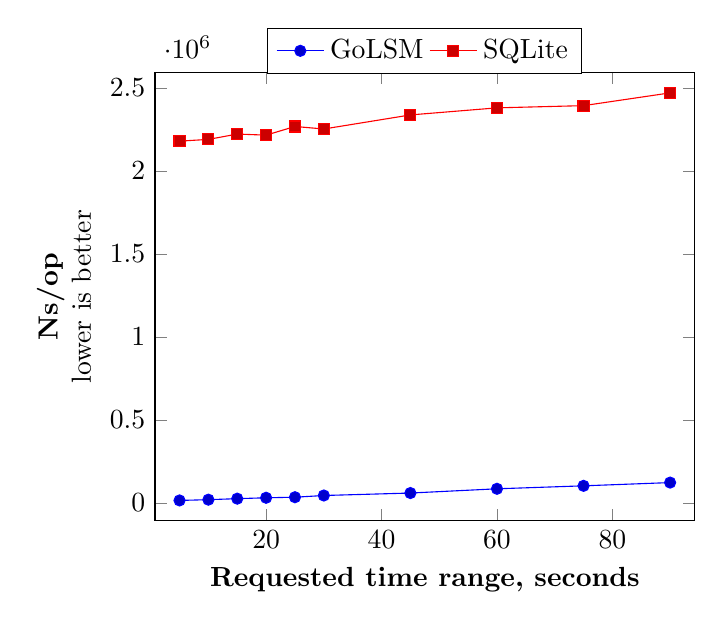
\begin{tikzpicture}
        % first provide your data as table, so later the data can
        % easily be accessed for various stuff
        \pgfplotstableread{
            x    y  z
5 14164				    2179781
10 18772			    2190392
15 24835			    2222522
20 30221			    2216021
25 33592			    2268216
30 43931			    2253056
45 58727			    2337832
60 84315			    2380516
75 102221			    2393851
90 121761			    2470748
        }{\data}
    \begin{axis}[
        x tick style={/pgf/number format/1000 sep=},
	    ylabel style={align=center},	
	    ylabel = \textbf{Ns/op}\\lower is better,
	    xlabel style={align=center},	
	    xlabel = \textbf{Requested time range, seconds},
	    enlargelimits=0.05,
	    legend style={
	        at={(0.5,1.1)}, anchor=north,legend columns=-1
	    },
    ]
        % then your `\addplot commands change to
        \addplot table [x=x,y=y] {\data};
        \addlegendentry{GoLSM}
        \addplot table [x=x,y=z] {\data};
        \addlegendentry{SQLite}
    \end{axis}
\end{tikzpicture}
		}
		\caption{Reading from full range of data.}\label{fig4}
	\end{minipage}\hfill
	\begin{minipage}{0.48\textwidth}
		\centering
		\resizebox{\textwidth}{!}{%
			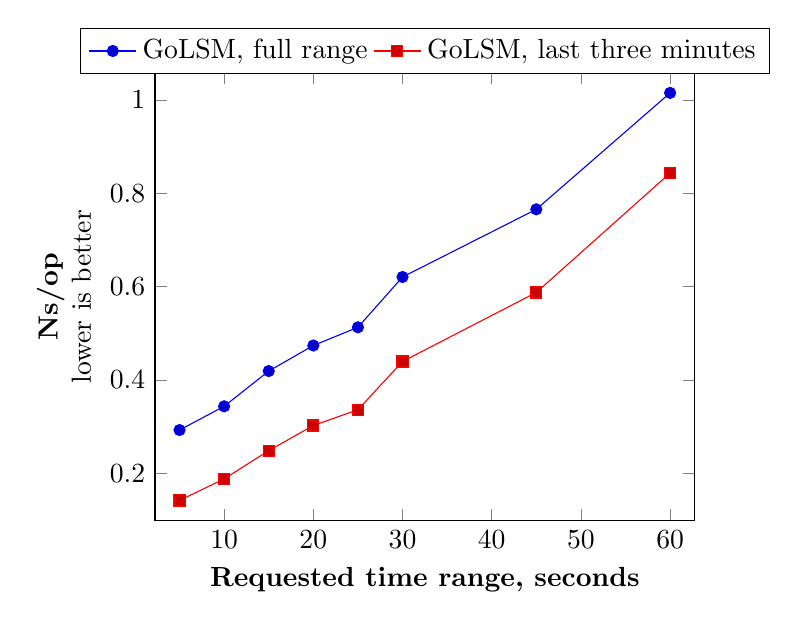
\begin{tikzpicture}
        % first provide your data as table, so later the data can
        % easily be accessed for various stuff
        \pgfplotstableread{
            x    y  z
5	29245	14164
10	34331	18772
15	41885	24835
20	47359	30221
25	51261	33592
30	62037	43931
45	76538	58727
60	101490	84315
        }{\data}
    \begin{axis}[
        x tick style={/pgf/number format/1000 sep=},
	    ylabel style={align=center},	
	    ylabel = \textbf{Ns/op}\\lower is better,
	    xlabel style={align=center},	
	    xlabel = \textbf{Requested time range, seconds},
	    enlargelimits=0.05,
	    legend style={
	        at={(0.5,1.1)}, anchor=north,legend columns=-1
	    },
    ]
        % then your `\addplot commands change to
        \addplot table [x=x,y=y] {\data};
        \addlegendentry{GoLSM, full range}
        \addplot table [x=x,y=z] {\data};
        \addlegendentry{GoLSM, last three minutes}
    \end{axis}
\end{tikzpicture}
		}
		\caption{Difference in GoLSM speed on the latest data.}\label{fig5}
	\end{minipage}
\end{figure}

If the data retrieval pattern is retrieving only the latest data, increasing the capacity of $C_0$ can drastically improve reading performance and reduce the reading load on the persistent disk storage.

\subsection{Writing linear data}

This benchmark measures the write time for various time ranges. While the data is linear the minimal timestamp of the next data batch to be written is always more than the maximum timestamp of the previously written batch. It means, for each SST within the GoLSM engine the data is only appended to the end of the SST file without the need to redo the sorting of the SST file. The results of this benchmark are available in Figure~\ref{fig6}.

\begin{figure}[!htb]
	\begin{minipage}{0.48\textwidth}
		\centering
		\resizebox{\textwidth}{!}{%
			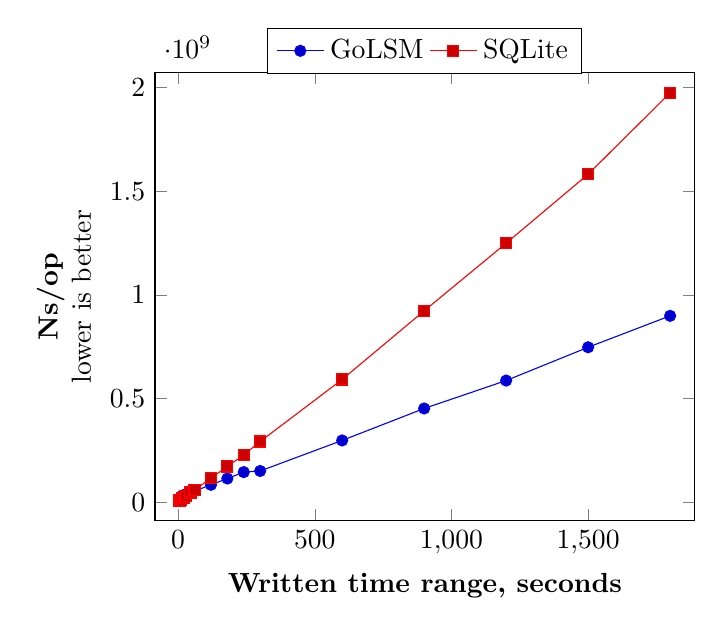
\begin{tikzpicture}
        % first provide your data as table, so later the data can
        % easily be accessed for various stuff
        \pgfplotstableread{
            x    y  z
5 15645901			    9353729
10 22956983			    11181460
15 32283634			    19307910
20 34011973			    21123025
25 33267746			    28927692
30 39930080			    30805858
45 49632256			    47978279
60 54524124			    59648520
120 84668307			    116531430
180 115137807			    173160076
240 146032654			    228964797
300 151417281			    293465746
600 298689957			    592581370
900 452684093			    923305824
1200 587385346			    1249406072
1500 747870163			    1582051745
1800 899311404			    1974174575

        }{\data}
    \begin{axis}[
        x tick style={/pgf/number format/1000 sep=},
	    ylabel style={align=center},	
	    ylabel = \textbf{Ns/op}\\lower is better,
	    xlabel style={align=center},	
	    xlabel = \textbf{Written time range, seconds},
	    enlargelimits=0.05,
	    legend style={
	        at={(0.5,1.1)}, anchor=north,legend columns=-1
	    },
    ]
        % then your `\addplot commands change to
        \addplot table [x=x,y=y] {\data};
        \addlegendentry{GoLSM}
        \addplot table [x=x,y=z] {\data};
        \addlegendentry{SQLite}
    \end{axis}
\end{tikzpicture}
		}
		\label{figure}{(a) Over big range}
	\end{minipage}\hfill
	\begin{minipage}{0.48\textwidth}
		\centering
		\resizebox{\textwidth}{!}{%
			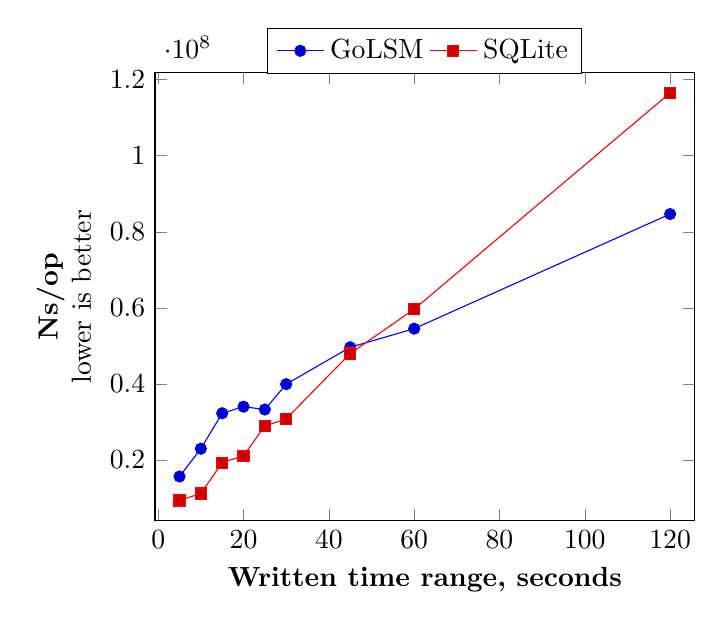
\begin{tikzpicture}
        % first provide your data as table, so later the data can
        % easily be accessed for various stuff
        \pgfplotstableread{
            x    y  z
5 15645901			    9353729
10 22956983			    11181460
15 32283634			    19307910
20 34011973			    21123025
25 33267746			    28927692
30 39930080			    30805858
45 49632256			    47978279
60 54524124			    59648520
120 84668307			    116531430

        }{\data}
    \begin{axis}[
        x tick style={/pgf/number format/1000 sep=},
	    ylabel style={align=center},	
	    ylabel = \textbf{Ns/op}\\lower is better,
	    xlabel style={align=center},	
	    xlabel = \textbf{Written time range, seconds},
	    enlargelimits=0.05,
	    legend style={
	        at={(0.5,1.1)}, anchor=north,legend columns=-1
	    },
    ]
        % then your `\addplot commands change to
        \addplot table [x=x,y=y] {\data};
        \addlegendentry{GoLSM}
        \addplot table [x=x,y=z] {\data};
        \addlegendentry{SQLite}
    \end{axis}
\end{tikzpicture}
		}
		\label{figure}{(b) Over small range}
	\end{minipage}
	
	\caption{Writing linear data.}\label{fig6}
\end{figure}

In Figure~\ref{fig6}, (a) it is clearly seen that GoLSM writes data twice as fast as SQLite over the big time range that is being written.  However, in Figure~\ref{fig6}, (b) for the small time range the GoLSM is actually slower. The reason for this is that for LSM was measured the time until the data is actually written to the commit log, and not directly to the SST files; and when the amount of entries in the commit log reaches a certain threshold, it has to be transferred to the SST, causing spikes in write time. However, for big time ranges being written this overhead is not important compared to generally slow batch inserts to SQLite. 

It is worth mentioning that for inserting to SQLite it is necessary to construct the SQL Insert statement that involves converting a double value to string. This operation is extremely slow for big batch inserts (a batch of 10 tags for 30 minutes is 18000 points), and using ORM such as GORM does not improve the situation.

\subsection{Writing randomized data}

This benchmark measures the write time for various time ranges, while the data is random, there are no guarantees that all of the next batch timestamps are bigger than the timestamps of the previously written batch. So the batches could occur before or after one another in terms of their timestamps. It means each time when the data is transferred from the commit log file to SST files the engine has to resort the whole SST file, slowing down the writing process. The results of this benchmark are available in Figure~\ref{fig7}. The comparison of writing the data to LSM when the data is either linear or randomized is available in Figure~\ref{fig8}.

\begin{figure}[!htb]
	\begin{minipage}{0.48\textwidth}
		\centering
		\resizebox{\textwidth}{!}{%
			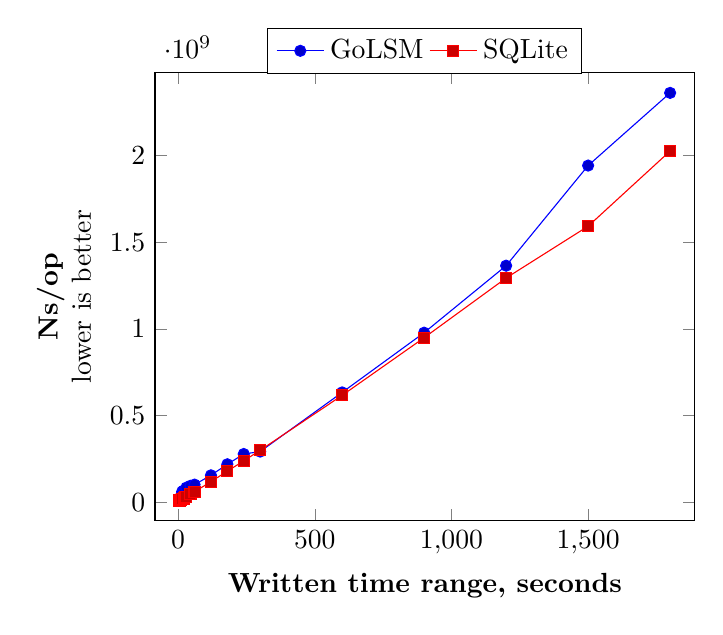
\begin{tikzpicture}
        % first provide your data as table, so later the data can
        % easily be accessed for various stuff
        \pgfplotstableread{
            x    y  z
5 20066750			    9514015
10 34790230			    10956443
15 61277403			    19290607
20 66074549			    20865090
25 63925416			    28999975
30 83572878			    30478476
45 94080339			    48656675
60 100926498			    59882936
120 154617448			    117794298
180 218391345			    178663220
240 277609792			    238031796
300 291599762			    299054072
600 633156270			    616109936
900 977887157			    948873690
1200 1364639379			    1293479495
1500 1942545058			    1592474416
1800 2362087783			    2026594877


        }{\data}
    \begin{axis}[
        x tick style={/pgf/number format/1000 sep=},
	    ylabel style={align=center},	
	    ylabel = \textbf{Ns/op}\\lower is better,
	    xlabel style={align=center},	
	    xlabel = \textbf{Written time range, seconds},
	    enlargelimits=0.05,
	    legend style={
	        at={(0.5,1.1)}, anchor=north,legend columns=-1
	    },
    ]
        % then your `\addplot commands change to
        \addplot table [x=x,y=y] {\data};
        \addlegendentry{GoLSM}
        \addplot table [x=x,y=z] {\data};
        \addlegendentry{SQLite}
    \end{axis}
\end{tikzpicture}
		}
		\caption{Writing randomized data.}\label{fig7}
	\end{minipage}\hfill
	\begin{minipage}{0.48\textwidth}
		\centering
		\resizebox{\textwidth}{!}{%
			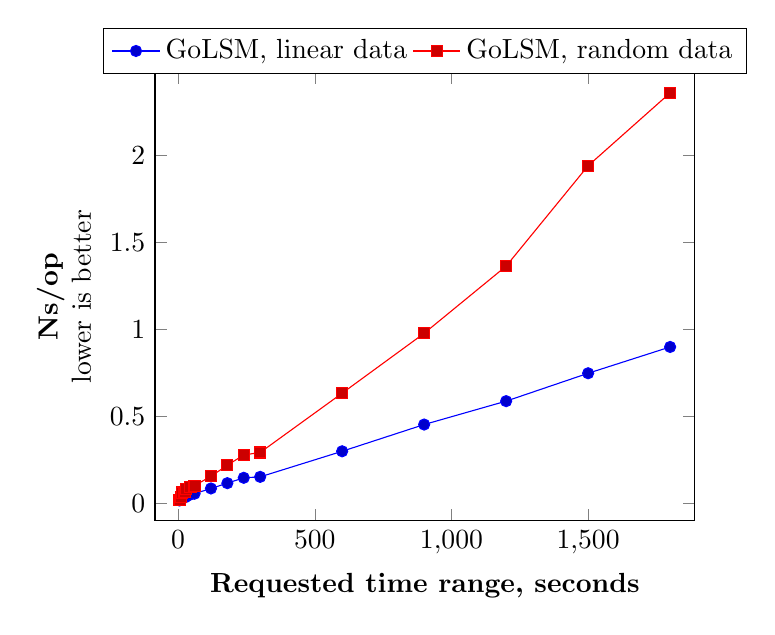
\begin{tikzpicture}
        % first provide your data as table, so later the data can
        % easily be accessed for various stuff
        \pgfplotstableread{
            x    y  z
5	15645901	20066750
10	22956983	34790230
15	32283634	61277403
20	34011973	66074549
25	33267746	63925416
30	39930080	83572878
45	49632256	94080339
60	54524124	100926498
120	84668307	154617448
180	115137807	218391345
240	146032654	277609792
300	151417281	291599762
600	298689957	633156270
900	452684093	977887157
1200	587385346	1364639379
1500	747870163	1942545058
1800	899311404	2362087783

        }{\data}
    \begin{axis}[
        x tick style={/pgf/number format/1000 sep=},
	    ylabel style={align=center},	
	    ylabel = \textbf{Ns/op}\\lower is better,
	    xlabel style={align=center},	
	    xlabel = \textbf{Requested time range, seconds},
	    enlargelimits=0.05,
	    legend style={
	        at={(0.5,1.1)}, anchor=north,legend columns=-1
	    },
    ]
        % then your `\addplot commands change to
        \addplot table [x=x,y=y] {\data};
        \addlegendentry{GoLSM, linear data}
        \addplot table [x=x,y=z] {\data};
        \addlegendentry{GoLSM, random data}
    \end{axis}
\end{tikzpicture}
		}
		\caption{Difference in GoLSM speed when writing linear and randomized data.}\label{fig8}
	\end{minipage}
\end{figure}

As seen in Figure~\ref{fig7}, the overhead of resorting the SST files on every data write is so big that it outperforms the slow batch inserts to SQLite. The comparison of the data writes with this overhead to data writes without the overhead is in Figure~\ref{fig8}. When the timestamps of the data are always linearly increasing, shows that the inserts are almost up to three times slower on large time range writes (747870163 ns/op, or 747 ms, for writing 25 minutes of linear data, and 1942545058 ns/op, or 1942 ms, for writing 25 minutes of randomized data).